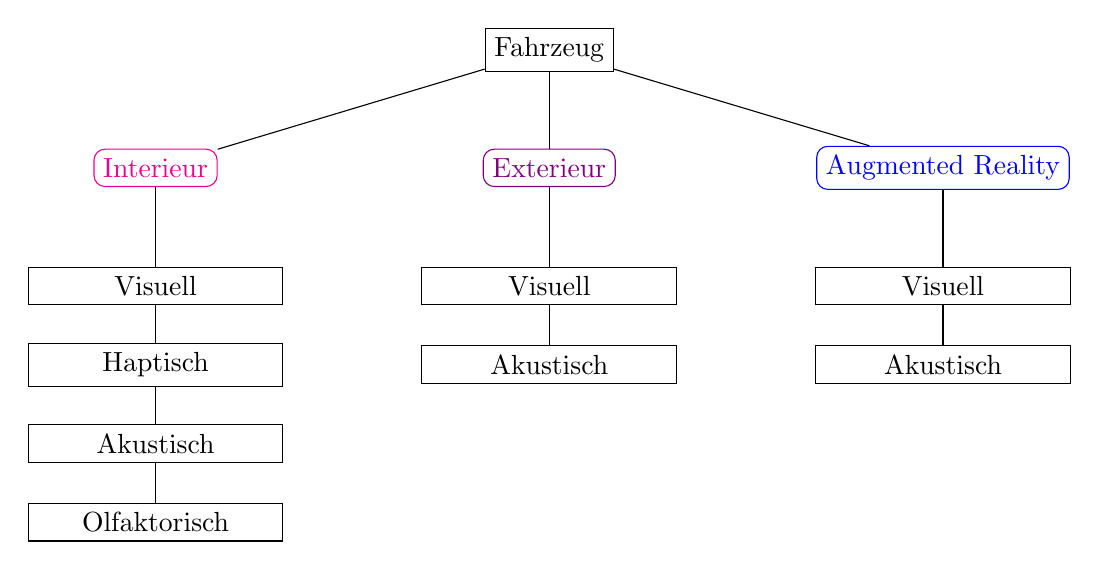
\begin{tikzpicture}[first style/.style={rectangle, draw, rounded corners, align=center}, steuer style/.style={draw, rectangle, align=center}, second/.style={draw, rectangle, align=center, text width=3cm}]
	\node[steuer style] (S1) at (0, 3) {Fahrzeug};
	\node[first style, magenta] (S2) at (-5, 1.5) {Interieur};
	\node[first style, violet] (S3) at (0, 1.5) {Exterieur};
	\node[first style, blue] (S4) at (5, 1.5) {Augmented Reality};
	\node[second] (S5) at (-5, 0) {Visuell};
	\node[second] (S6) at (-5, -1) {Haptisch};
	\node[second] (S7) at (-5, -2) {Akustisch};
	\node[second] (S8) at (-5, -3) {Olfaktorisch};
	\node[second] (S9) at (0, 0) {Visuell};
	\node[second] (S10) at (0, -1) {Akustisch};
	\node[second] (S11) at (5, 0) {Visuell};
	\node[second] (S12) at (5, -1) {Akustisch};
	\foreach \x in {2,...,4}
	\draw (S1) -- (S\x);
	\draw (S2) -- (S5);
	\draw (S5) -- (S6);
	\draw (S6) -- (S7);
	\draw (S7) -- (S8);
	\draw (S3) -- (S9);
	\draw (S9) -- (S10);
	\draw (S4) -- (S11);
	\draw (S11) -- (S12);
\end{tikzpicture}